
\documentclass[draft]{../agujournal2019}
\usepackage{url} \usepackage{lineno}
\usepackage[inline]{../trackchanges} \usepackage{soul}
\usepackage{amsmath}
\usepackage{pifont}  \linenumbers

\draftfalse


\journalname{Water Resources Research}


\begin{document}
\justify


\graphicspath{{/Users/songshgeo/Documents/VSCode/WGRegimes_YRB_2020/figures}}
\title{Identifying regime transitions for water governance at the Yellow River Basin, China}









\authors{
      Shuang Song\affil{1},
      Shuai Wang\affil{1},
      Xutong Wu\affil{1},
      yongping Wei\affil{2},
      Graeme S. Cumming\affil{3},
      Yue Qin\affil{4},
      Xilin Wu\affil{5},
      Bojie Fu\affil{1,5}
}


\affiliation{1}{
      State Key Laboratory of Earth Surface Processes and Resource Ecology,
      Beijing Normal University,
      Beijing, 100875, Beijing, China.
}
\affiliation{2}{
      School of Earth and Environmental Sciences,
      The University of Queensland,
      Brisbane, 4067, QLD, Australia.
}
\affiliation{3}{
      ARC Centre of Excellence for Coral Reef Studies,
      James Cook University,
      Townsville, 4811, QLD, Australia.
}
\affiliation{4}{
      College of Environmental Sciences and Engineering,
      Peking University,
      Beijing, 100875, Beijing, China.
}
\affiliation{5}{
      State Key Laboratory of Urban and Regional Ecology,
      Research Center for Eco-Environmental Sciences,
      Chinese Academy of Sciences,
      Beijing, 100875, Beijing, China.
}





\correspondingauthor{Shuai Wang}{shuaiwang@bnu.edu.cn}





\begin{keypoints}
      \item An Integrated Water Governance Index (IWGI) was devised to identify regime shifts in water governance practices.
      \item The study interprets the transformation of water governance within a rapidly evolving large river basin -the Yellow River Basin.
      \item A novel approach was developed to analyze interconnections between water governance, hydrosocial transition, and human-water relationships.
\end{keypoints}




\begin{abstract}
Water governance determine ``who gets water, when, and how'' in most large river basins.
Shifts in water governance regimes from natural to social-ecological or ``hydrosocial'' carry profound implications for human wellbeing; identifying regime changes in water governance is critical to navigating social-ecological transitions and guiding sustainability.
We characterized water governance along with the three main aspects - stress, purpose, and allocation - to develop a quantitative Integrated Water Governance Index (IWGI) at a basin scale.
Applying the IWGI to the rapidly-changing Yellow River Basin (YRB) in China clarifies shifts in water governance between massive supply, transformation governance, and adaptation-oriented regimes.
In the YRB, the underlying causes of regime shifts were increasing water supply and demand before the governance transformation and re-allocation and regulation after the change.
The IWGI offers a comprehensive and straightforward approach to linking water governance regimes to sustainability, providing valuable insights into hydrosocial transitions.
\end{abstract}

\section*{Plain Language Summary}
Missing governance means missing sustainability. However, the lack of a comprehensive but straightforward approach to identifying the changes in water governance presents a challenge for efforts to underpin it. Therefore, we choose indicators for the corresponding aspects (water stress, water services purpose, and water allocation) and combine them into an integrated water governance index (IWGI) to analyze long-term changes in a large river basin.


\section{Introduction}\label{sec1}

Water, being ``at the centre of the planetary drama of the Anthropocene'', is essential not only for earth system processes but also in supporting development and human well-being~\cite{gleeson2020a,gleeson2020b}.
As an integral part of earth system governance, successful water governance requires a deep understanding of changes in the complex relationships between humans and water~\cite{ahlstrom2021,biermann2012,steffen2020}.
Human activities stemming from our reliance on water have profoundly modified the natural water cycle, resulting in rivers that are dominated by a hybrid of social and natural drivers~\cite{sivapalan2012,qin2014a,abbott2019}.
Facing transitions from natural to human-dominated regimes, many big river basins worldwide (which are hot spots of civilization and economic growth) are urgently in need of more effective water governance~\cite{best2019,dibaldassarre2019}.

Water governance encompasses the political, social, economic, and administrative systems that regulate water use and management, dictating ``who gets water, when and how''~\cite{lasswell2018,allan2001}.
In this context, the United Nations Development Programme (UNDP) suggests that water governance determines water usage across three core aspects: ``When and what water to use?'' (stress), ``How does water provide different services for human well-being?'' (purpose), and ``Who can use water equally and efficiently?'' (allocation)~\cite{mariajacobson2013}.
Research into index-based water governance assessment generally fall into two categories: those that focus on water systems, and those that concentrate on governance systems.
On one hand, studies on governance systems typically employ an qualitative assessment to demonstrate what practices influence water governance, e.g., the OECD framework~\cite{oecd2018a}.
For quantitative studies, due to the lack of comprehensive and detailed information on key components for water governance assessment, these studies often resort to proxy datasets of human activities to create simpler indices~\cite{varis2019,huggins2022a}.
On the other hand, studies focusing on water systems utilize intuitive indices to encapsulate the outcomes of governance, like the most widely concerned -water stress has been far developed by incorporating human's regulation step by step.
Specifically, traditional water stress index only demands and supply~\cite{gleick1996}, water scarcity index by involving storage~\cite{damkjaer2017}, and the even more integrated SFV-index includes flexibility~\cite{qin2019}.
Despite their usefulness, these water stress indices tend not to provide a comprehensive characterization of water governance, as they overlook the social aspect of water usage, i.e., the purpose and allocation of water use.
As a solution, we propose an integrated water governance index (IWGI) that factors in regional water use allocations and sectoral water use purpose, thereby offering a more comprehensive quantification of governance outcomes.

The impetus for developing this new index lies in the evolving practices of water governance driven by a blend of social and natural influences.
Firstly, climate change impacts on current water yield, coupled with escalating demands from economic activities and the need for water storage development, intensify water stress~\cite{qin2019,wada2014,huang2021}.
Secondly, the purpose of water in serving human well-being is witnessing a shift in trade-offs. The balance between provisioning uses (such as drinking water and food production) and non-provisioning uses (like energy production) is tilting, reflecting changes in societal needs and values~\cite{liu2017,florke2018,jaeger2019}.
Thirdly, the allocation of water across a basin is not solely determined by regional socio-economic and environmental contexts but is also increasingly influenced by systematic regulations~\cite{schmandt2021,speed2013}.
As we transition towards a human-dominated regime, these three interlinked aspects -stress, purpose, and allocation, are undergoing substantial changes.
Assessing them separately could lead to systematic failures in water governance, highlighting the need for a more integrated approach in evaluating water governance practices.

A critical step in understanding the successes and failures of water governance is to identify the different regimes that underpin it~\cite{kjellen2015, grafton2013}.
Regimes of water governance, the general guidelines of governing practices, arise within linked human-water systems (based on management, institutions, and exploitation) to create local equilibria in social-ecological structures and functions~\cite{falkenmark2021,bressers2013,loch2020,pahl-wostl2007}.
For example, under a human-dominated regime, reservoirs make water stress easier to be alleviated because of flexibility; growing energy and industrial demands make water services purposes lopsided to non-provisioning sectors; conveyance systems make water allocation more planned (Figure~\ref{fig:framework}~A)
However, the lack of a comprehensive but straightforward approach to identifying changes in water governance regimes represents a challenge for efforts to enhance the sustainability of water resource use.
Filling this gap, which is the aim of this paper, is essential for the appropriate alignment of human and water systems.


\begin{figure*}[!ht]
	\centerline{
		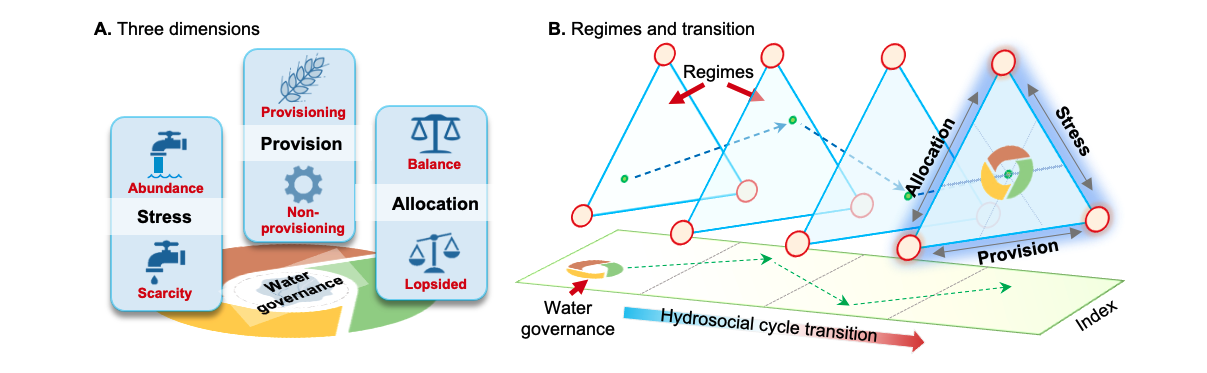
\includegraphics[width=1.1\linewidth]{main/framework.png}
	}
	\caption{
		\textbf{A.} Identifying the water governance regimes in transitions of a hydrosocial cycle with an integrated water governance index (IWGI). Water stress (S), purposes of water services (P), and water allocation (A) are three aspects to be considered.
		For example, reservoir construction (\ding{172} and \ding{173}) can relieve local water stress; The development of intensive irrigated agriculture (\ding{174}) and growth of energy industrial demand (\ding{175}) will change the purpose of water use; The water delivery system controls water allocation (\ding{176} and \ding{177}) within the basin system.
		\textbf{B.} Therefore, the methodology is to combine three aspects' corresponding indicators, and then an abrupt change of the IWGI can indicate a regime shift in water governance.
	}\label{fig:framework}
\end{figure*}


The Yellow River Basin (YRB), which contains the fifth-largest and most sediment-rich river in the world, needs integrated water governance because of geological and human history~\cite{mostern2021,best2019}.
Since the 1960s, governance practices such as reservoirs, levees, and conservation measures have contained the issues troubled by thousands of years of high sediment loads~\cite{wang2016a,song2020}.
However, new challenges such as decreased streamflows and water depletions occurred in more recent times, followed by different water governance practices like water use regulation and water transfer across basins~\cite{wang2019c}.
Today, it is still impossible to completely solve water stress, trade-offs between ecosystem services, or lopsided development in different regions in the YRB to the satisfaction of all actors~\cite{wohlfart2016}.
Governance challenges induced by environmental, economic, social, and political factors have resulted in YRB being among the most intensively-governed large river basins worldwide~\cite{nickum2021}.
Identifying regime shifts in water governance within the YRB can thus provide crucial insights into rapidly-changing big river basins and how governance may respond to meeting challenges to their sustainability.

Here, we depict three aspects of water governance -stress, purpose and allocation with corresponding indicators (see methods) and thus develop an Integrated Water Governance Index (IWGI) by equally weighting them, to indicate results from water governance (see Figure~\ref{fig:framework}~B).
Then, by applying the index to a typical rapid-changing big river basin (the YRB), we show how IWGI helps detect and describe complicated water governance regimes comprehensively but straightforwardly.
Following synthetic analyses of the changes in water demand, supply, economic outcomes, and institutions, we interpret the leading causes of the regime shifts.
Finally, we propose a general regime transition schema that offers a practical guideline for a coordinated approach to exploring the challenges faced by big river basin governance.

\section{Materials and Methods}\label{sec11}


To develop a comprehensive and straightforward approach to identifying water governance regimes. First, we constructed the Integrated Water Governance Index (IWGI) based on three aspects (Stress, Purpose, and Allocation, see Figure~\ref{fig:framework}). Then, we analyzed the changes in the IWGI from 1965 to 2013 using change point detection methods. The normalized indicator for each dimension affects the IWGI by changing trends and contributions.

\subsection{Integrated Water Governance Index (IWGI)}

As shown in the framework Figure~\ref{fig:framework}, the IWGI combines the three aspects (Stress, Purpose, and Allocation) of water governance:
	\begin{equation}
		Transformation \propto S*P*A
	\end{equation}

	We selected an indicator ($I_x$, $x=S$, $P$, or $A$, corresponding to stress, purpose, and allocation, respectively) to quantify the aspects effectively. Then, the above equation was transformed into a natural logarithm to facilitate calculation:
	\begin{equation}
		Transformation \propto \ln(I_S) + \ln(I_P) + \ln(I_A)
	\end{equation}

	Then, the Integrated Water Governance Index (IWGI) is an average of the normalized indicators $I'_x$:
	\begin{equation}
		IWGI = (I'_S + I'_P + I'_A) / 3
	\end{equation}

	where $I'_x$ is calculated by Min-Max normalization of $I_x$ (thus ranges from zero to one):
	\begin{equation}
		I'_x = (I_x - I_{x, \min}) / (I_{x, \max} - I_{x, \min})
	\end{equation}

	Since the IWGI essentially comprises by three aspects' indicator with same weights, its prerequisite is to keep the same data source for each indicator throughout time, to ensure time series continuity.
	However, vary data sources can be used when estimating the specific indicator or cross different indicators, which makes IWGI a flexible framework for substituted indicators.

	\subsubsection{Indicator of stress (IS)}
	We used the scarcity-flexibility-variability (SFV) water stress index proposed by \citeA{qin2019} to evaluate water stress.
	This indicator integrates the share of runoff being consumed, the share of consumption in these inflexible categories and the historical variability of runoff weighted by storage capacity~\cite{qin2019}, where impacts from both management measures and climate changes are included.
The SFV-index, which has many applications, is the most comprehensive index of water stress we know.

	Based on the hydrological and economic context of YRB, four second-level regions are divided (Source Region, Upper Region, Middle Region, and Lower Region, see \textit{Supporting Information Section~S1}).
	For the whole YRB, the indicator of water stress $I_S$ is the average of all regions' SFV-index:
	\begin{equation}
		I_S = \frac{1}{4} * \sum_{i=1}^4 SFV_{i}
	\end{equation}

	Where $SFV_i$ is the scarcity-flexibility-variability (SFV) index of region $i$. By taking water flexibility and variability into account, the SFV focus more on dynamic responses to water resources in a developing perspective, which is a valid metric of temporal changes in water stresses~\cite{qin2019}. To apply this method, we need to combine three metrics: scarcity, flexibility and variability.
	In all the equations following, $R_{i, avg}$ is the average runoff in region $i$, $RC_i$ is the total storage capacities of reservoirs in the region $i$, $R_{i, std}$ is the standard deviation of runoff in the region $i$.

	First, for scarcity, $A_{i, j}$ is the total water consumption as a proportion of regional multi-year average runoff volume in year $j$ and region $i$ (in this study, four regions in the YRB, \textit{Supporting Information Section S1}):
	\begin{equation}
		A_{i, j} = \frac{WU_{i,j}}{R_{i, avg}}
	\end{equation}

	Second, for flexibility, $B_{i, j}$ is the inflexible water use $WU_{inflexible}$ (i.e.\ for thermal power plants or humans and livestock) as a proportion of average multi-year runoff, in year $i$ and region $j$:
	\begin{equation}
		B_{i, j} = \frac{WU_{i, j, inflexible}}{R_{i, avg}}
	\end{equation}

	Finally for variability, the capacity of the reservoir and the positive effects of storage on natural runoff fluctuations are also considered.
	\begin{gather}
	C_i = C1_i * (1 - C2_i) \\
	C1_{i, j} = \frac{R_{i, std}}{R_{i, avg}} \\
	C2_{i} = \frac{RC_{i}}{R_{i, avg}}, \ if RC < R_{i, avg} \\
	C2_{i} = 1, \ if RC >= R_{i, avg}
	\end{gather}

	Finally, assuming three metrics (scarcity, flexibility and variability) have the same weights, we can calculate the $SFV$ index after normalizing them:
	\begin{gather}
		V = \frac{A_{normalize} + B_{normalize} + C_{normalize}}{3}\\
		a = \frac{1}{V_{\max} - V_{\min}};\\
		b = \frac{1}{V_{\min} - V_{\max}} * V_{\min}\\
		SFV = a * V + b
	\end{gather}

	\subsubsection{Indicator of purpose (IP)}
	To quantify purpose $I_P$, we used provisioning purpose shares (PPS) of water use as an indicator. While provisioning purpose water use ($WU_{pro}$) includes domestic, irrigated, and livestock water uses, non-provisioning purpose water use ($WU_{non-pro}$) includes industrial and urban services water uses. We calculated the PPS by:
	\begin{equation}
		PPS = \frac{WU_{pro}}{WU_{pro} + WU_{non-pro}}
	\end{equation}

	In this study, we consider livestock water use, rural and urban domestic water use, and agricultural water use as provisioning water because they directly service for survival. Others are non-provisioning: services and industrial water use because they mainly service the economy.

	\subsubsection{Indicator of allocations (IA)}
	To describe allocations $I_A$, we designed an indicator based on entropy, called Allocation Entropy Metric (AEM), which measures the degree of evenness in water allocation:

	\begin{equation}
		I_A = AEM = \sum_{i=1}^N - \log(p_{i}) * p_{i}
	\end{equation}

	where $p_{i}$ is the proportion of regional water use in $i$ to water use of the whole basin (here, $N=4$ considering divided regions in the YRB, see \textit{Supporting Information S1}).

	\subsection{Change points detection}
		We applied the Pettitt (1979) approach to detect change-points of IWGI within continuous data, since this method has no assumptions about the distribution of the data~\cite{pettitt1979}.
		It tests $H0$: The variables follow one or more distributions with the exact location parameter (no change) against the alternative: a change point exists.
		Mathematically, when a sequence of random variables is divided into two segments represented by $\mathrm{x}_{1}, \mathrm{x}_{1}, \ldots, x_{t_{0}}$ and $x_{t_{0}+1}, x_{t_{0}+2}, \ldots, x_{T}$, if each segment has a common distribution function, i.e., $F_1(x)$, $F_2(x)$ and $F_1(x) \neq F_2(x)$, then the change point is identified at $t_0$. To achieve the identification of change point, a statistical index $U_{t,T}$ is defined as follows:

		\begin{equation}
			U_{t, T} = \sum_{i=1}^t\sum_{j=t+1}^T sgn(X_i - X_j), 1 \leq t < T
		\end{equation}

		where:
		\begin{equation}
			\operatorname{sgn}(\theta)= \begin{cases}1 & \text { if } \theta>0 \\ 0 & \text { if } \theta=0 \\ -1 & \text { if } \theta<0\end{cases}
		\end{equation}

		The most probable change point $\tau$ is found where its value satisfies $K_{\tau} = \max|U_{t, T}|$ and the significance probability associated with value $K_{\tau}$ is approximately evaluated as:
		\begin{equation}
			p=2 \exp \left(\frac{-6 K_{\tau}^{2}}{T^{2}+T^{3}}\right)
		\end{equation}
		Given a certain significance level $\alpha$, if $p < \alpha$, we reject the null hypothesis and conclude that $x_{\tau}$ is a significant change point at level $\alpha$.

We used $\alpha = 0.001$ as the threshold level of the p-value, meaning that the probability of a statistically significant change-point judgment being valid was more than $99.9\%$. We divided the series into two at that point and analyzed each series separately until all significant change points were detected. Though two break points in the main text with $\alpha = 0.001$, the threshold from $0.0005$ to $0.05$ does not affect our results, and the breakpoints we identified are robust (see Figure~S6).

	\subsection{Datasets}\label{sec:datasets}

	For calculating IWGI, three datasets were used: reservoirs, measured runoff, and water uses.
	The reservoir dataset was collected by~\citeA{wang2019c}, which introduced includes the significant new reservoirs built in the YRB since 1956.
	Among all the reservoirs, YRCC labelled the ``major reservoirs'' which were constructed mainly for regulating and managing (see \url{http://www.yrcc.gov.cn/hhyl/sngc/}).
	In addition, annual measured runoff data was collected from the Yellow River Sediment Bulletin (\url{http://www.yrcc.gov.cn/nishagonggao/}) and four controlling stations are measuring different reaches of the Yellow River (see Supporting Informations Section~S1).
	The water resources use dataset was from National Long-term Water Use Dataset of China (NLWUD) published by \citeA{zhou2020}, which includes water uses, water-consuming economic variables, and water use intensities by sectors the prefectures level.
	We determined the prefectures belong to the YRB by filtering the NLWUD dataset with a threshold of $95\%$ intersected area.

	For analyzing its causes of changing water, irrigated area, gross added values of industry and services, and water use intensities data were also from NLWUD dataset~\cite{zhou2020}.
	Besides, two water governance policies datasets are used: laws data and ``big events'' documents dataset.
	Data of laws were collected from~\citeA{yellowriverwaterconservancycommission2010}, which reviewed all important laws at the basin scale related to the Yellow River from the last century.
	The original documents of ``big events'' related to the Yellow River come from the YRCC, the agency at the basin scale, which recorded and compiled these events (\url{http://www.yrcc.gov.cn/hhyl/hhjs/}).

	Finally, we calculated the IWGI from 2001 to 2017 (the latest) in the Supporting Information Section S4 for robustness test with another water use dataset from Yellow River Water Resources Bulletin (\url{http://www.yrcc.gov.cn/zwzc/gzgb/gb/szygb/}).
 \section{Results}\label{sec2}
\subsection{Water governance regimes}\label{Res.1}

\begin{figure*}[ht!]
	\centering
	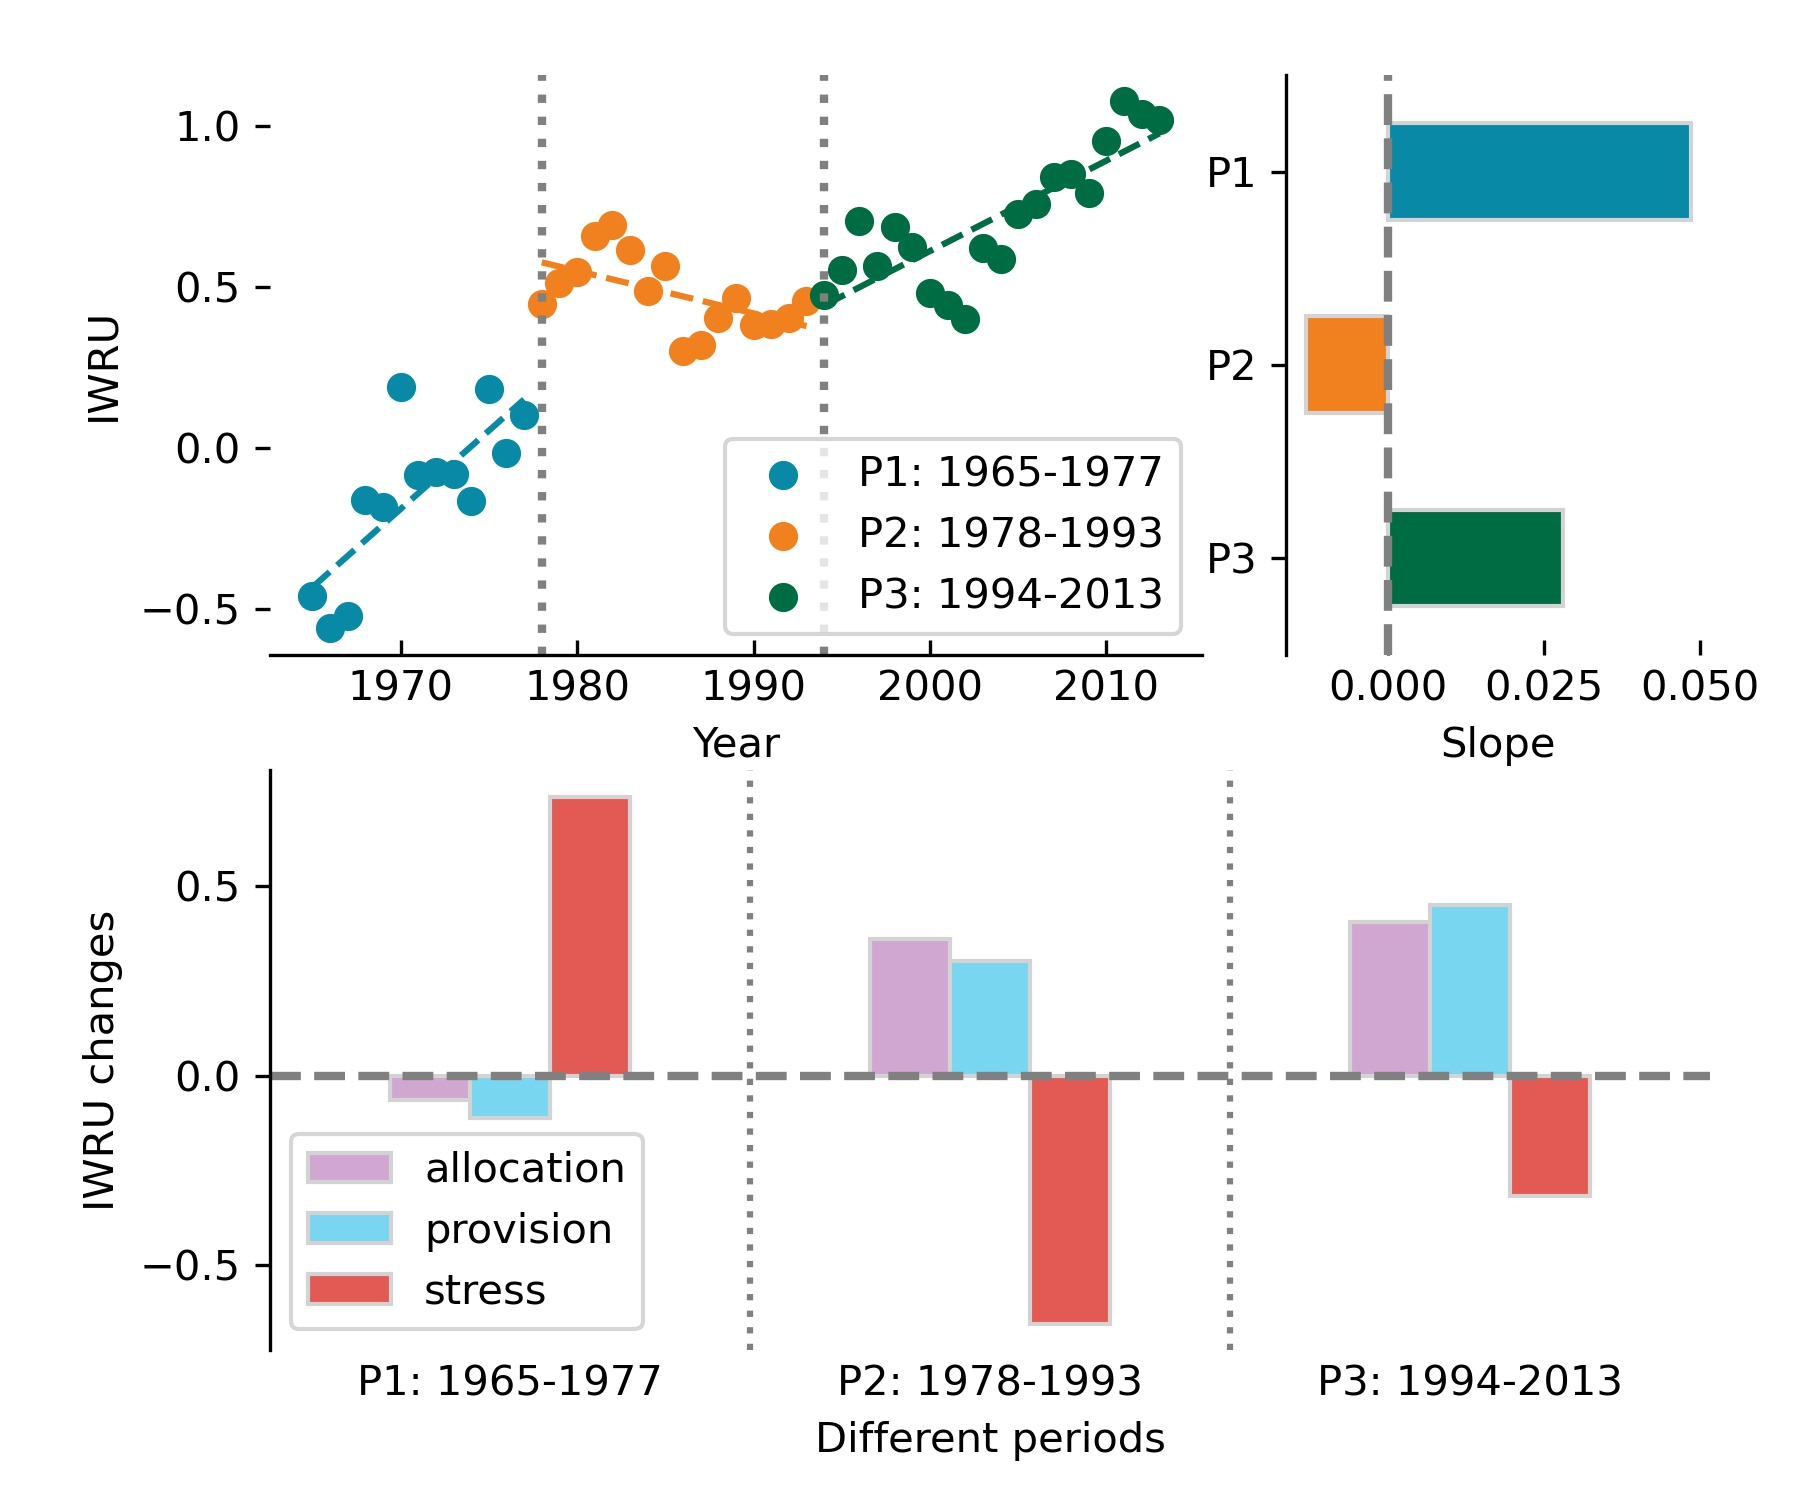
\includegraphics[width=0.9\linewidth]{main/index.jpg}
	\caption{Changes in the IWGI index and corresponding water governance regimes: P1: $1965 \sim 1978$, P2: $1979 \sim 2001$, and P3: $2002 \sim 2013$.
	\textbf{A,} detecting change points of IWGI and contributions from each indicator. Two significant change points ($p<0.001$) occurred in 1978 and 2001.
	\textbf{B,} correlation of trends between the IWGI and the indicators.
	\textbf{C,} across three indicators, changing components of the IWGI, whose directions shifts between different regimes.
	}\label{fig:IWGI}
\end{figure*}

Two significant breakpoints divide the changes in the IWGI into three periods, with different contributions from three aspects (Figure~\ref{fig:IWGI}A).
In the first period (P1, $1965 \sim 1978$), the IWGI decreased rapidly.
While the indicator of purpose and allocation contributed more to the IWGI ($49.45\%$ and $34.95\%$ on average, respectively), the remarkable downward trend correlates significantly ($p<0.01$) to the decreasing allocation and stress indicators (Figure~\ref{fig:IWGI}B).
In the second period (P2, $1979 \sim 2001$), the increasing stress indicator significantly ($p<0.01$) contributed to the upward IWGI, while the allocation and purpose indicators played negative roles in changing the IWGI.\
During the third period (P3, $1995 \sim 2013$), while the stress indicator kept its most prominent share in contributions ($57.11\%$ on average), the increased allocation indicator and decreased purpose indicator changed the regime.
Taken together, the overall features of the three aspects in different periods are relative to a directional change in the combination of three aspects (Figure~\ref{fig:IWGI}C).

\subsection{Causes of the regime shifts}\label{Res.2}

\begin{figure*}[th!]
	\centering
	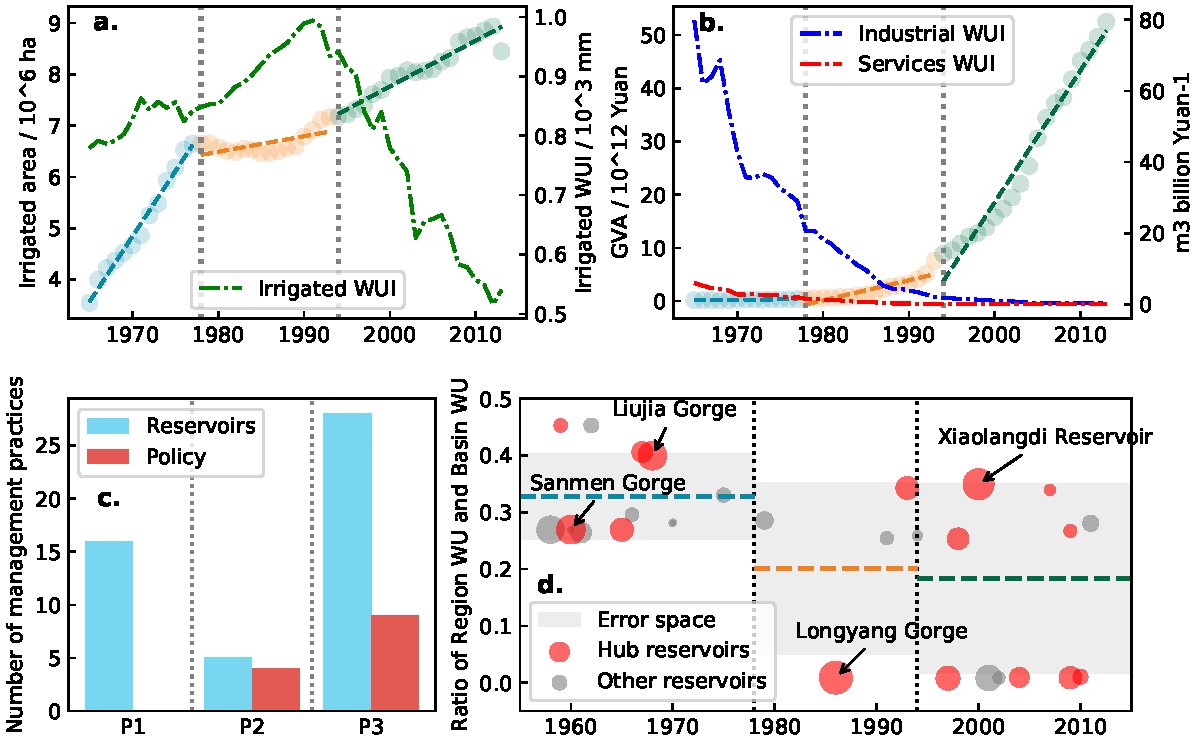
\includegraphics[width=0.9\linewidth]{main/causes.pdf}
	\caption{
		Causes of water governance regime shifts in the YRB.\
		\textbf{A.} Changes in the total irrigated area (orange line) and water use intensity ($WU/A$, water use divided by the irrigated area, the green dot line).
		\textbf{B.} Changes in gross values added (GVA) of industry and services (blue line) and their water use intensities ($WU/GVA$ WU divided by the GVA, the red dot line).
		\textbf{C.} Completed time of each new reservoir and their located region's water use (LWU) percentages as a proportion of the total basinal water use (BWU) at that time. Dashed lines denote average of these percentages in different regimes. Red circles (Major Reservoirs) denote the reservoirs mainly for managing and regulating the whole basin.
		The size of each circle indicates the magnitude of its water storage capacity.
		\textbf{D.} Social atmosphere (red triangles) and national-level governance policies (the circles, different colours denote signed by different state agencies). The light grey bars count official documents related to the YRB on a basinal scale (the Yellow River Events).
	}\label{fig:Causes}
\end{figure*}

The underlying causes of changes in the IWGI are different in the two regime shifts.
Changing water demands and supply were critical to the shift between P1 and P2.
As the dominant water demand during the P1, the area of irrigated agriculture in the YRB expanded rapidly at a rate of $0.25*10^6~ha/yr$ (Figure\ref{fig:Causes}~A), simultaneously supported by increasing supply through the construction of reservoirs.
Ensuing the P2, however, the expansion of irrigated areas slowed down, and industry and services gradually took off (Figure\ref{fig:Causes}~A and B).
Then, the efficiency of water use changed obviously from P2 to P3.
Not only did irrigated areas continue to expand slowly during the P3 (Figure\ref{fig:Causes}~A), but industry and urban services also assumed a more vital economic role (represented by Gross Added Values, GVA) (Figure~\ref{fig:Causes}~B).
Because of increased efficiency, however, they both experienced significant declines in water use for a unit irrigated area or unit production (Figure~\ref{fig:Causes}~A and Figure~\ref{fig:Causes}~B).
As a result, the differences between sectors and regions in water use reduced while the total water stress steadily remained high during the P3 (Figure~\ref{fig:IWGI}A).

Environmental context, social atmosphere, and policies played roles in all three periods.
We calculated the ratios of regional and basinal water use for each reservoir (R/B ratio) (Figure~\ref{fig:Causes}C), with a higher ratio representing a potential role in water supply rather than basinal regulations.
Under the banner of ``conquering nature'' most of the reservoirs were built in regions with high water demands during the P1 (R/B ratios were significantly higher ($p<0.01$, see Figure~\ref{fig:Causes}C)).
Ensuing the P2, the number of new reservoirs decreased but boosted their role in water regulating and management (more red circles in Figure~\ref{fig:Causes}~C, and larger water conveyance variability in Supporting Informations Figure~S7).  Basin policies significantly increased, rigorously controlled the allocation of water (Figure~\ref{fig:Causes}D, $p<0.01$).
During the P3, authorities proposed more national-level water governance policies under the guidance of the national strategy ``environmental regulation'' (Figure~\ref{fig:Causes}D).
The regime shift from P1 to P2 is in line with the increasing water supply and demands; while driven by regulatory policies and efficiency enhancement under stable water stress from P2 to P3.


\section{Discussion}\label{sec12}

Water governance gradually becomes a national or international concern from a primarily local concern because large river basins are critical sources of ecosystem services, economic development, and human well-being~\cite{best2019,best2020}.
As tele-coupling raises additional water governance challenges in an increasingly tightly-connected world, regime shifts in water governance align with different human-water relationships~\cite{diaz2019}.
The process echoes how societies have been proposed to change governance practices by enhancing their adaptive capacity in the hydrosocial cycle~\cite{loch2020,turton1999}, and the IWGI quantitatively identifies this transition.
It is vital for scientists and decision-makers to recognize the changing governance challenges because models, institutions, engineering, and approaches developed under one regime are not necessarily applicable under a different regime~\cite{reyers2018}.

In the case of the YRB, our results show that there have been three distinct governance regimes; we named them: a massive supply regime (P1: $1965 \sim 1978$), a governance transforming regime (P2: $1979 \sim 2001$), and an adaptation oriented regime (P3: $2002 \sim 2013$) (Figure~\ref{fig:IWGI}).
During the massive supply regime with lower water stress ($1965 \sim 1978$ in the YRB), water governance thus tended to boost water supply for services (mainly provisioning purposes then -livestock and crops) by constructing reservoirs and channels (Figure~\ref{fig:Causes}~B).
As the Chinese slogan ``human will conquer nature'' suggested then, however, the enhancement of water supply did not align with irreversible changes in the human-water relationship; it drastically increased water demand with little consideration for ecological conservation~\cite{zhou2020}.
The rapid expansion of irrigated farmland and water diversion facilities in the same decade brought the overburdened YRB close to a critical point (Figure~\ref{fig:Causes}), where increasing supply to meet demand was impractical~\cite{loch2020}.
Use of over $80\%$ of the surface water since 1972 has led to frequent river depletion, causing additional ecological issues such as wetland shrinkage and declines in biodiversity~\cite{wang2019c}.
In addition, since water stress also limited the growing industrial economy, the existing modes of water governance led to a social-ecological crisis~\cite{wohlfart2016}.

The start of the governance transforming regime (P2: $1979 \sim 2001$) coincided with rising competition for water use after the ``reform and opening-up'' (Figure~\ref{fig:Causes}~C).
The results from the YRB mirror those of the theoretical analysis: continuous increases in water demand when the basin's total supply is stable can follow substantial changes in governance regime and a rapid enhancement in overall social adaptive capacity~\cite{loch2020}.
As a pioneer in shifting governing institutions, the YRB triggered institutional changes during this regime. These include, for example, slowing the growth of irrigated acreage and leading water-saving infrastructure (Figure~\ref{fig:Causes}); creation of China's first water quota scheme, and the creation of a preliminary cross-boundary water transfer plan~\cite{wang2019e,long2020,nickum2021}.
Consequently, although water stress remained and increased (due to reducing streamflow and flexibility), the last depletion of the Yellow River in 1999 led to a climax in this transformation in water governance~\cite{wang2019e}.

The ensuing adaptation-oriented regime (P3: $2002 \sim 2013$) involved a significant societal shift in adapting to stable high water stress.
Partially because of changed climate~\cite{han2023,liu2020c}, the runoff of the YRB was significantly lower than before when the overall water uses remained stable, which was an important reason for the rise of water stress in this stage (Supporting Informations Figure~S2 and Figure~S3).
Socio-economic trade-offs between water-dependent regions and sectors, however, played a more important role in this regime, so water governance had to achieve efficient water allocation while balancing different demands in the face of limited water supply~\cite{dalin2015,song2022}.
Widespread reconstruction of resources in different industries and regions led to calls for adaptation in water governance, using the urgent requirements of adjusting rigid quota shares from the previous regime as an example~\cite{wang2019e}.
Many national-level governance practices were proposed under the regime because the absence of such policies to support high-quality development became new a structural challenge for water governance~\cite{konar2019}.

In general, water governance of the YRB is among the most prominent example in the widespread transition to a hydrosocial cycle -``improving supply, transforming governance, and enhancing adaptation''.
To support water use in early stage (Figure~\ref{fig:summary}~A), strategies tend to manage natural water processes in order to maintain the provisioning (larger) and non-provisioning water (less).
At the later stage (Figure~\ref{fig:summary}~B), emphasis is governing across the whole basin, water governance practices are adaptively designed to meet the increasing needs of the socio-economic system and carried out.
With the above gradually shifting, the emergence of different regimes drives water governance challenges at a basin-scale: these were primarily economic and environmental before the transformation, but social and policy-related towards the end (Figure~\ref{fig:summary})~\cite{singh2019,porcher2019}.
In an analogy at a global scale, the resource challenges, represented by water shortage and water supplying difficulties, are mainly faced by undeveloped and developing basins~\cite{allan2019,speed2013,liu2012}.
Highly-controlled and developed basins (especially for transboundary rivers) must mainly resolve structural challenges, such as water disputes or lack of equity, and may be in urgent need of novel flexible, efficient sociopolitical governance structures~\cite{unep-dhi2016,mirumachi2015}.
Linking regime shifts to the governance challenges, the implementation of IWGI thus offers a comprehensive and straightforward way to interpret the intertwines between water governance and the hydrosocial transition.

Future's tightly intertwined socio-hydro interactions can lead water governance challenges even more complex and comprehensive, combining resources issues and structural barriers~\cite{huggins2022a}.
For example, climate change may alter water scarcity levels and make it more difficult to effectively use water due to extreme climate events, strengthening water stress and threatening infrastructures~\cite{liu2017, dibaldassarre2019}.
Additionally, adapting to climate change could lead to transformations~\cite{sachs2019,barnes2020}, prompting a reevaluation of governance strategies of social water usage (purpose and allocation) which is being increasingly altered by current regime transitions.
It may be difficult to exhaust what is considered in a good watershed governance strategy, but the IWGI at least gives us a sense of where the a river basin is heading and how challenged.

\begin{figure*}[htbp!]
	\centering
	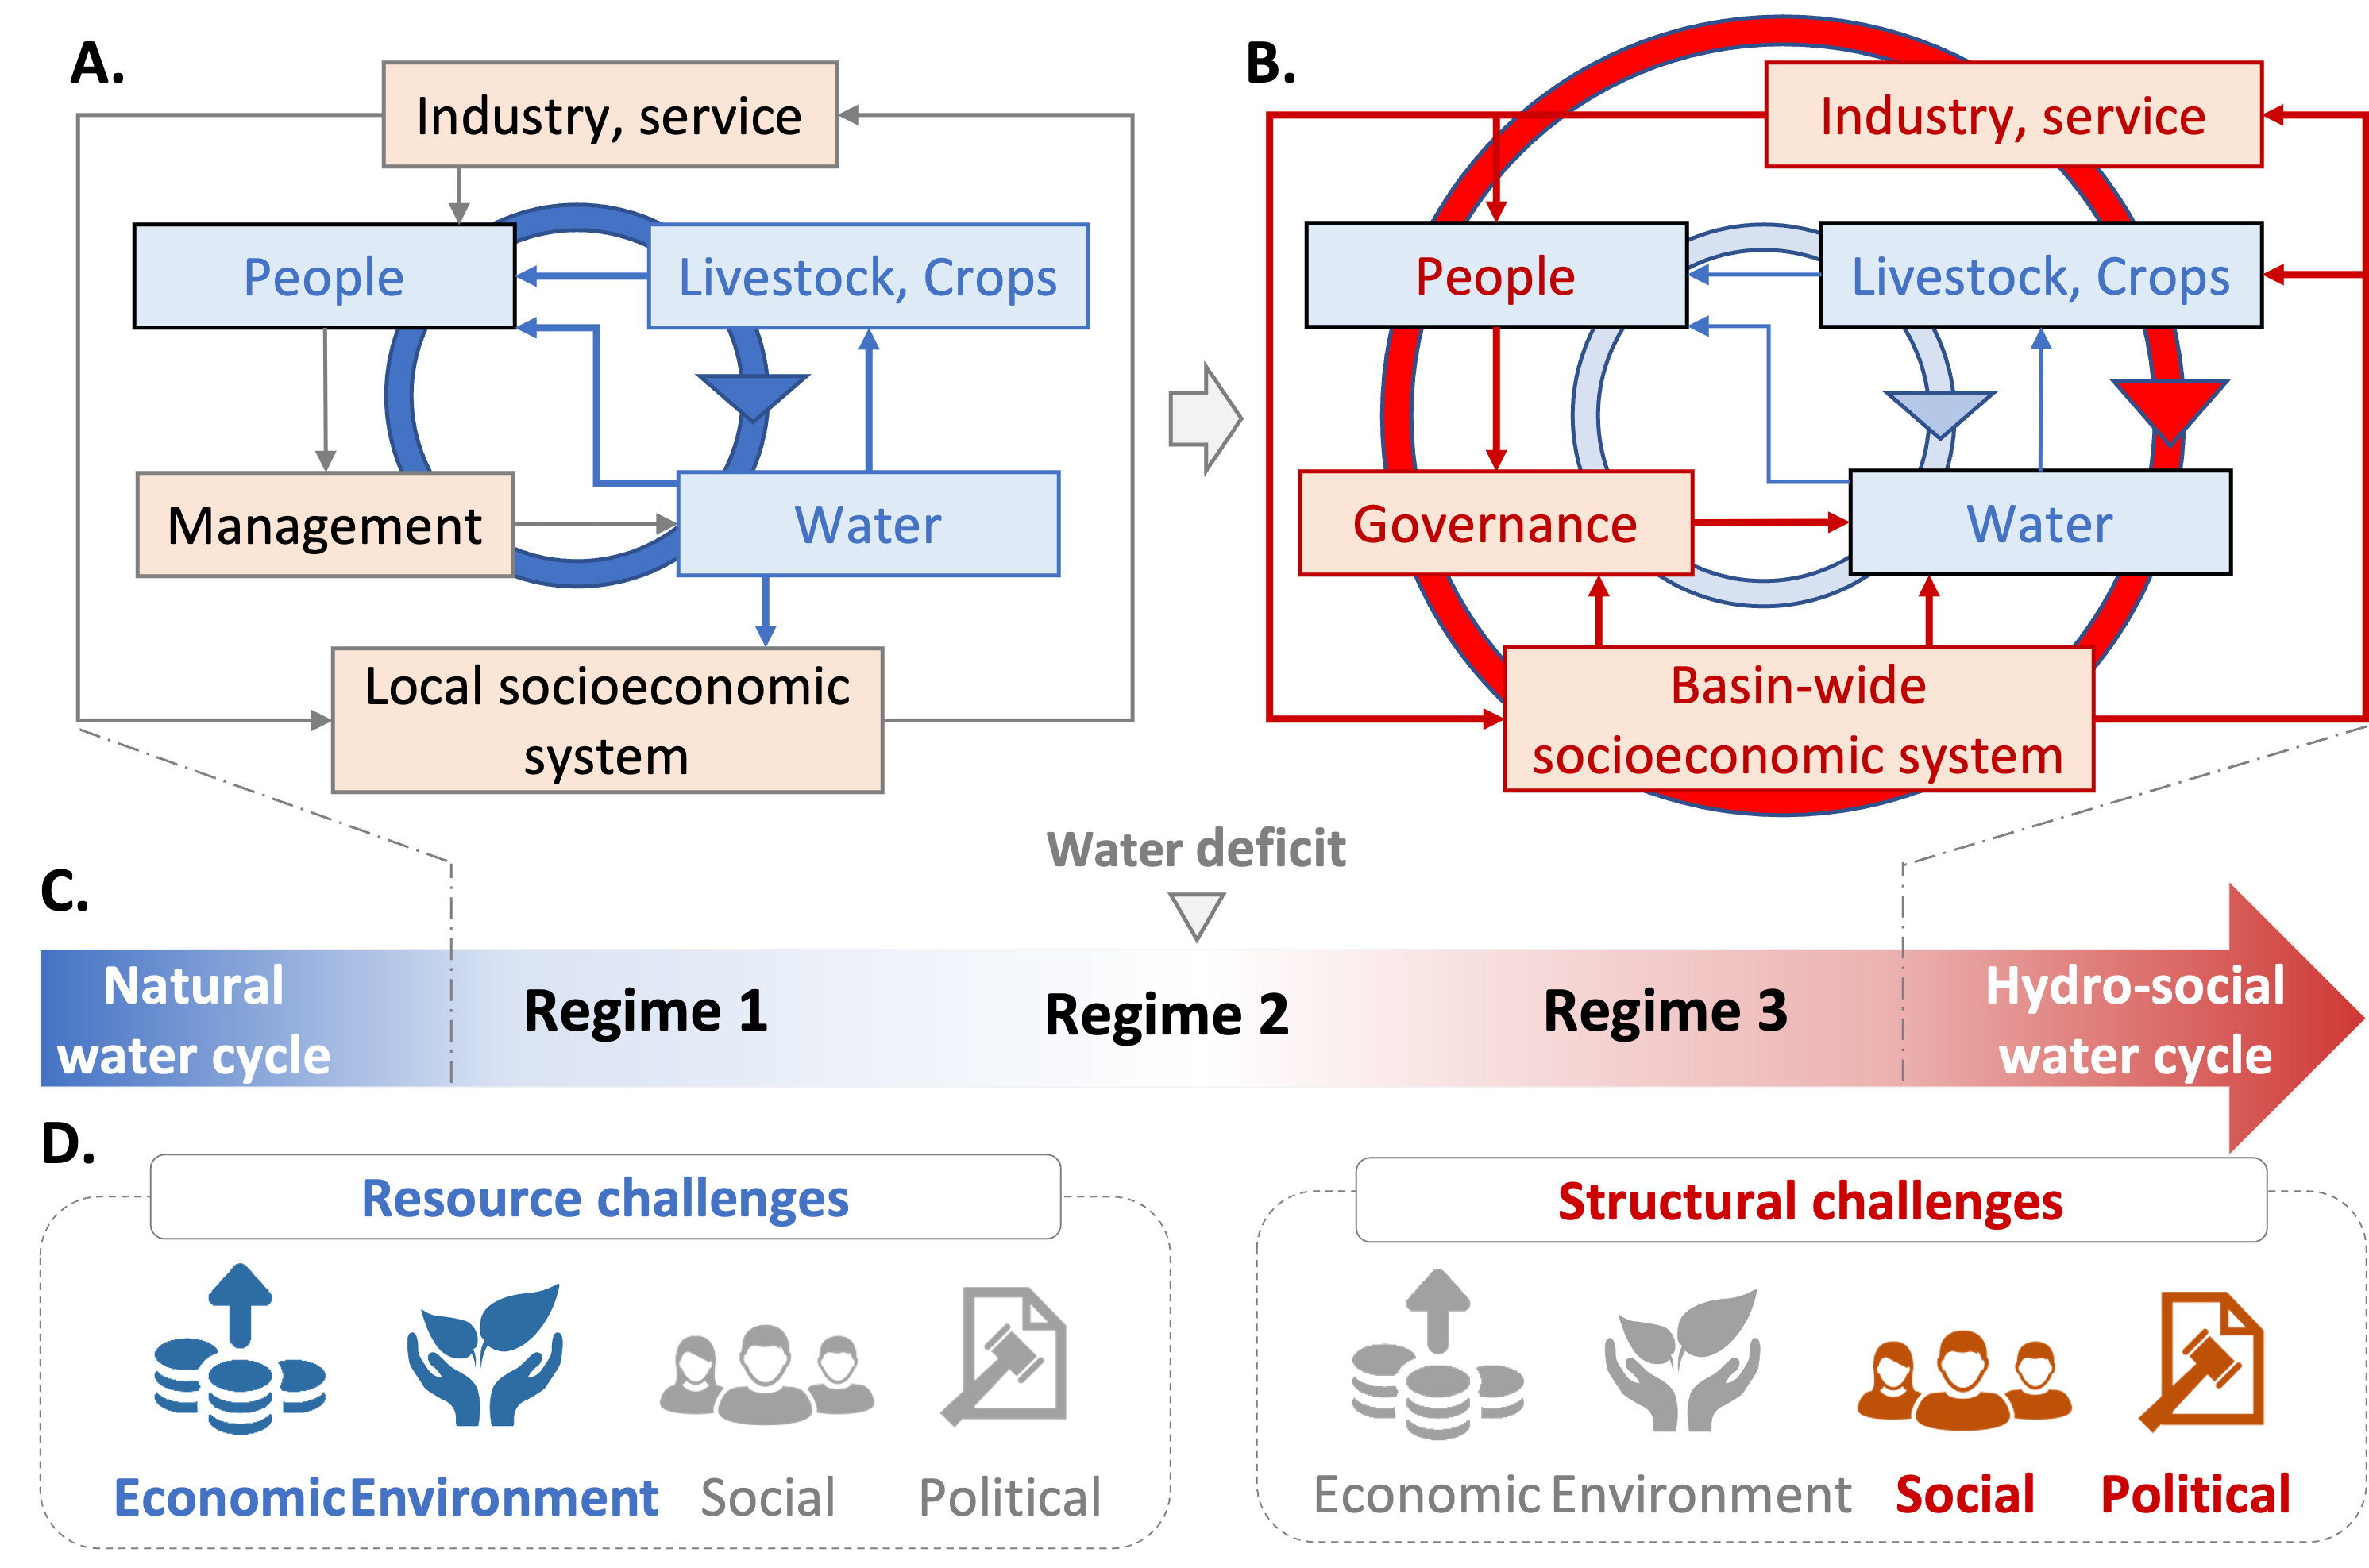
\includegraphics[width=0.8\linewidth]{main/transition.png}
	\caption{
		Transition schema in hydrosocial cycle and water governance regimes. The natural water cycle dominates blue pathways, while socio-economic feedback dominates red.
		The large circular arrows indicate the social and hydrological processes that dominate in different stages.
		Provisioning water includes water used by human, livestock and crops while non-provisioning water includes used by industry and service.
		The processes expressed in the graph mainly include: Water supports people in provisioning ways or influence/influenced socioeconomic systems as non-provisioning ways; People manage/govern water system based on their well-beings.
		The gray thick arrow represents weaker process, while the red arrow represents more significant one.
		\textbf{A.} As socio-economic systems develop, non-provisioning water demand increases; simultaneously, increased adaptive capacity by engineering allows people to manage water resources to alleviate water stress.
		\textbf{B.} With further growing socio-economic systems, trade-offs between provisioning-purpose and non-provisioning water use become prominent; a basin-wide socio-economic system requires more organized water governance.
		Thus, \textbf{C. the hydrosocial water cycle transition} correlates with the water governance regime shifts. The transformation governance regime shift occurs following the water deficit, with the rapid growth of adaptive capacity.
		\textbf{D. Water governance challenges} Through the transitional regimes, water governance faces primarily economic and environmental challenges but social and policy challenges later.
	}\label{fig:summary}
\end{figure*}


One of the main limitations in the approach is the lack of multi-sources data in long-term period worldwide, which means there is still a gap between comprehensively identifying and applying the IWGI widely.
We propose that all water governance issues, however, can change ``who gets water, when and how'' so monitoring such an integrated index is essential, even use simpler indicators.
We suggest that choices of indicators for different aspects can be adopted according to available datasets -e.g., replace the SFV-index (IA) with simpler scarcity index or proportion-based purpose indicator (IP) by complicated one.
Another limitation is the lack of latest datasets which is coherent with the historical datasets, so our analysis had to discontinued in 2013 despite potential shifts existing.
As a supplement, we examined IWGI framework with fewer datasets from different source in recent decades where showing no significant regime changes (supplementary Figure~\ref{fig:summary}).  Therefore, we suggest IWGI framework can be applied with adaptive indicators and flexible time series according to accessible datasets in future studies.

In today's world, regime shifts from natural to human-dominated seem likely to become increasingly widespread; comprehensive strategies to address governance challenges will have to become the core of complex human-water systems~\cite{cumming2018,cumming2014,jaeger2019}.
Although river basins have shown improvements in water management technologies and water use efficiency, many are still approaching local, regional, and planetary boundaries where human-water systems may collapse~\cite{gleeson2020, wang-erlandsson2022}.
A deeper understanding of governance that incorporates ideas of non-linear regime shifts and transformations should help shift the focus of governance towards maintaining the resilience of the basin’s social-ecological system and improving its sustainability~\cite{falkenmark2019}.

\section{Conclusion}\label{sec13}
Focusing on ``who gets water, when and how'', three aspects of water governance change along with the hydrosocial cycle transition: water stress, water services purpose, and water allocation.
We developed an Integrated Water Governance Index (IWGI) to detect regime shifts in water governance by integrating them. Applying the IWGI to a rapidly-changing large river basin (the Yellow River Basin, China), we interpret how water governance shifts between three regimes over half a century.
During the massive supply regime (P1: $1965 \sim 1978$), water governance tended to boost water supply by constructing reservoirs and channels in the YRB.\
Then, the start of the governance transforming regime (P2: $1979 \sim 2001$) coincided with rising competition for water use and led to institutional changes like water-saving improvements, water quota policies, and cross-boundary water transfer plans.
Last, adaptation-oriented regime (P3: $2002 \sim 2013$) with stable high water stress resulted in trade-offs and joint regulating between water-dependent regions and sectors.
Our approach quantitatively identifies the general schema for water governance regimes in the YRB, in line with previous theoretical analysis with a representative transition process.
Linking regime shifts to the underlying causes, the implementation of IWGI offers a comprehensive and straightforward way to interpret changes in intertwines of water governance, hydrosocial transition, and human-water relationships.
























\section*{Open Research Section}
All data used or analyzed during this study, including the reservoirs dataset, measured runoff, water uses datasets, laws, and big events are available under CC-BY 4.0 license~\cite{shuang_song_2023_7955500}.
Figures were made with Matplotlib version 3.7.1~\cite{Hunter:2007} and python-ternary version 1.0.8~\cite{pythonternary}.
These open sourced softwares are available under the Matplotlib license at \url{https://github.com/matplotlib/matplotlib} and the MIT license at \url{https://github.com/marcharper/python-ternary}, separately.


\acknowledgments
Funding was provided by the National Natural Science Foundation of China (CN) (Grant Nos. NSFC 42041007).

\bibliography{
../mybibtex.bib,
../others.bib
}


\end{document}
